% CREATED BY DAVID FRISK, 2015
\chapter{Theoretical Framework}

\lettrine[findent=2pt]{\fbox{\textbf{T}}}{ }his chapter introduces theory that is related to this study covering the areas of architectures in automotive domain, the two types of electrical architectures at VCG, and the proprietary tool Elektra that stores the low-level architectures. Theory of data collection method is also explained in this chapter.


\section{Architectures in automotive domain}
Proper architecture is necessary for designing and building modern vehicles which mostly are driven by electronics and software. Here are some related works that explain how it plays an important role in automotive domain.\\

Beeck \cite{Beeck} developed a modeling approach for development of software for ECUs at BMW Group, which supports the development of logical and technical architectures (high- and low-level architectures, respectively). The approach was developed based on the notation Unified Modeling Language for Real-Time (UML-RT) to compromise the complexity issue of developing, integrating, and maintaining software-intensive systems in vehicles. The logical architecture model is developed using UML-RT's capsule structure diagrams representing graphical system view of automotive functions. The technical architecture separated into software and hardware architectures is developed using UML-RT's component diagrams (for software) and deployment diagrams (for hardware). \\

For the logical architecture, the author created a UML-RT constructs and used them to model the architecture. From the meta-model (figure \ref{fig:beeck_metalmodel}), capsules, ports, protocols, signals, and connectors notations are used for modeling architectural artifacts. Capsules represent functions, while ports and protocols model function interfaces. A port is used to specify a communication point of a capsule. Each port has associated protocol, which contains two sets of signals: export and import. Connectors represent channels between function interfaces. \\

For the technical architectures, Components are used to model software components. Hardware components such as ECUs and sensors are modelled using UML-RT nodes. \\

The author, however, finds that still there are some issues regarding the use of UML-RT. One of the problems is, the set of UML-RT diagram notations is quite restricted. It is hard for ECU developers, who are familiar with non-object-oriented notations, to work with. In addition, the two protocols associated with ports do not meet requirements of some ECUs.

\begin{figure}[H]
\centering
\captionsetup{justification=centering}
\vspace{0cm}% Adjust vertical spacing here
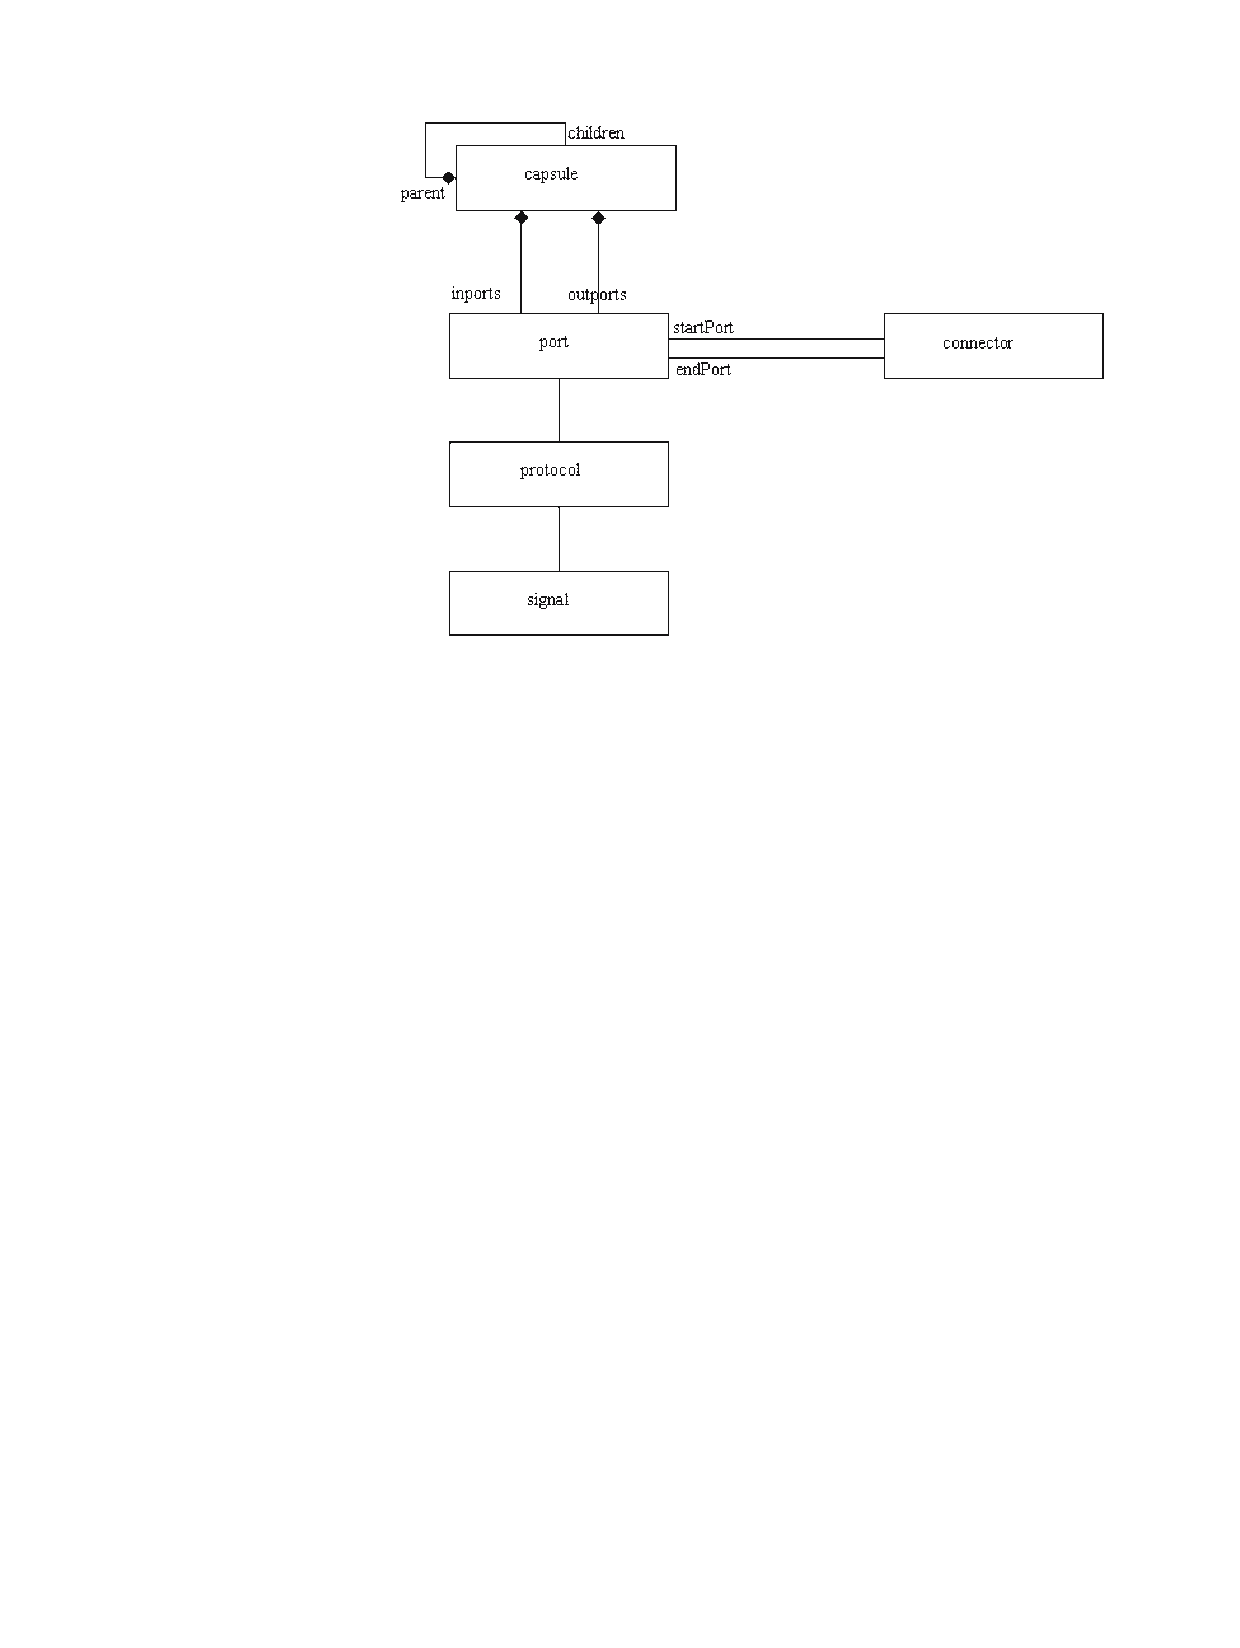
\includegraphics[width=0.55\linewidth]{figure/literatures/beeck_metalmodel.pdf}
\caption{Meta-model of UML-RT constructs for logical architecture \cite{Beeck}}
\label{fig:beeck_metalmodel}
\end{figure}

Grönniger et al. \cite{Grönniger} developed an approach for modelling logical architectures of automotive systems using views. Function nets which are valid Systems Modeling Language (SysML) Internal Block Diagrams (IBD) are used to model complete automotive functions and views which describe the environment and context of a certain aspect of function net. In addition to that, views can be used to model features in a self-contained way, and specify consistency conditions for consistency between a view and a function net.

\begin{figure}[H]
\centering
\captionsetup{justification=centering}
\vspace{0cm}% Adjust vertical spacing here
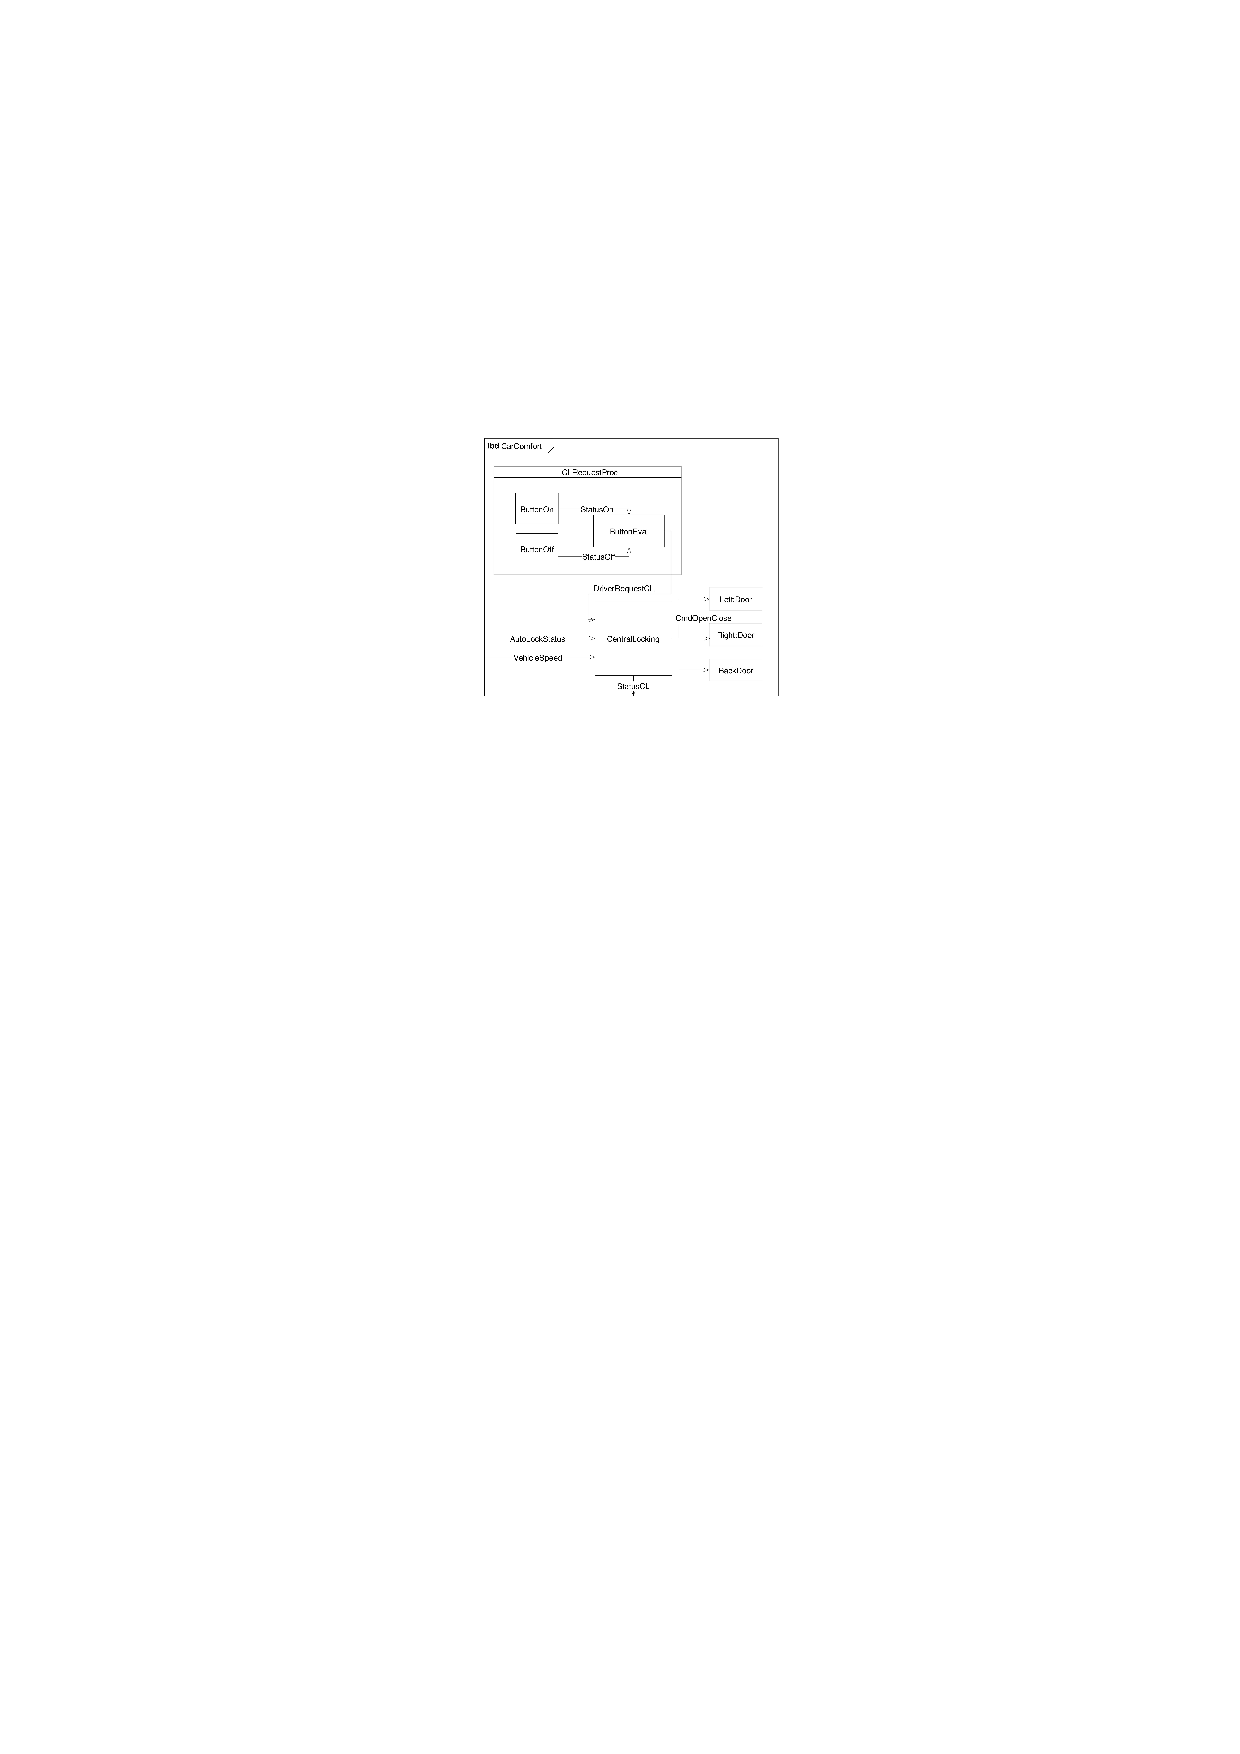
\includegraphics[width=0.35\linewidth]{figure/literatures/gronniger_sysml1.pdf}
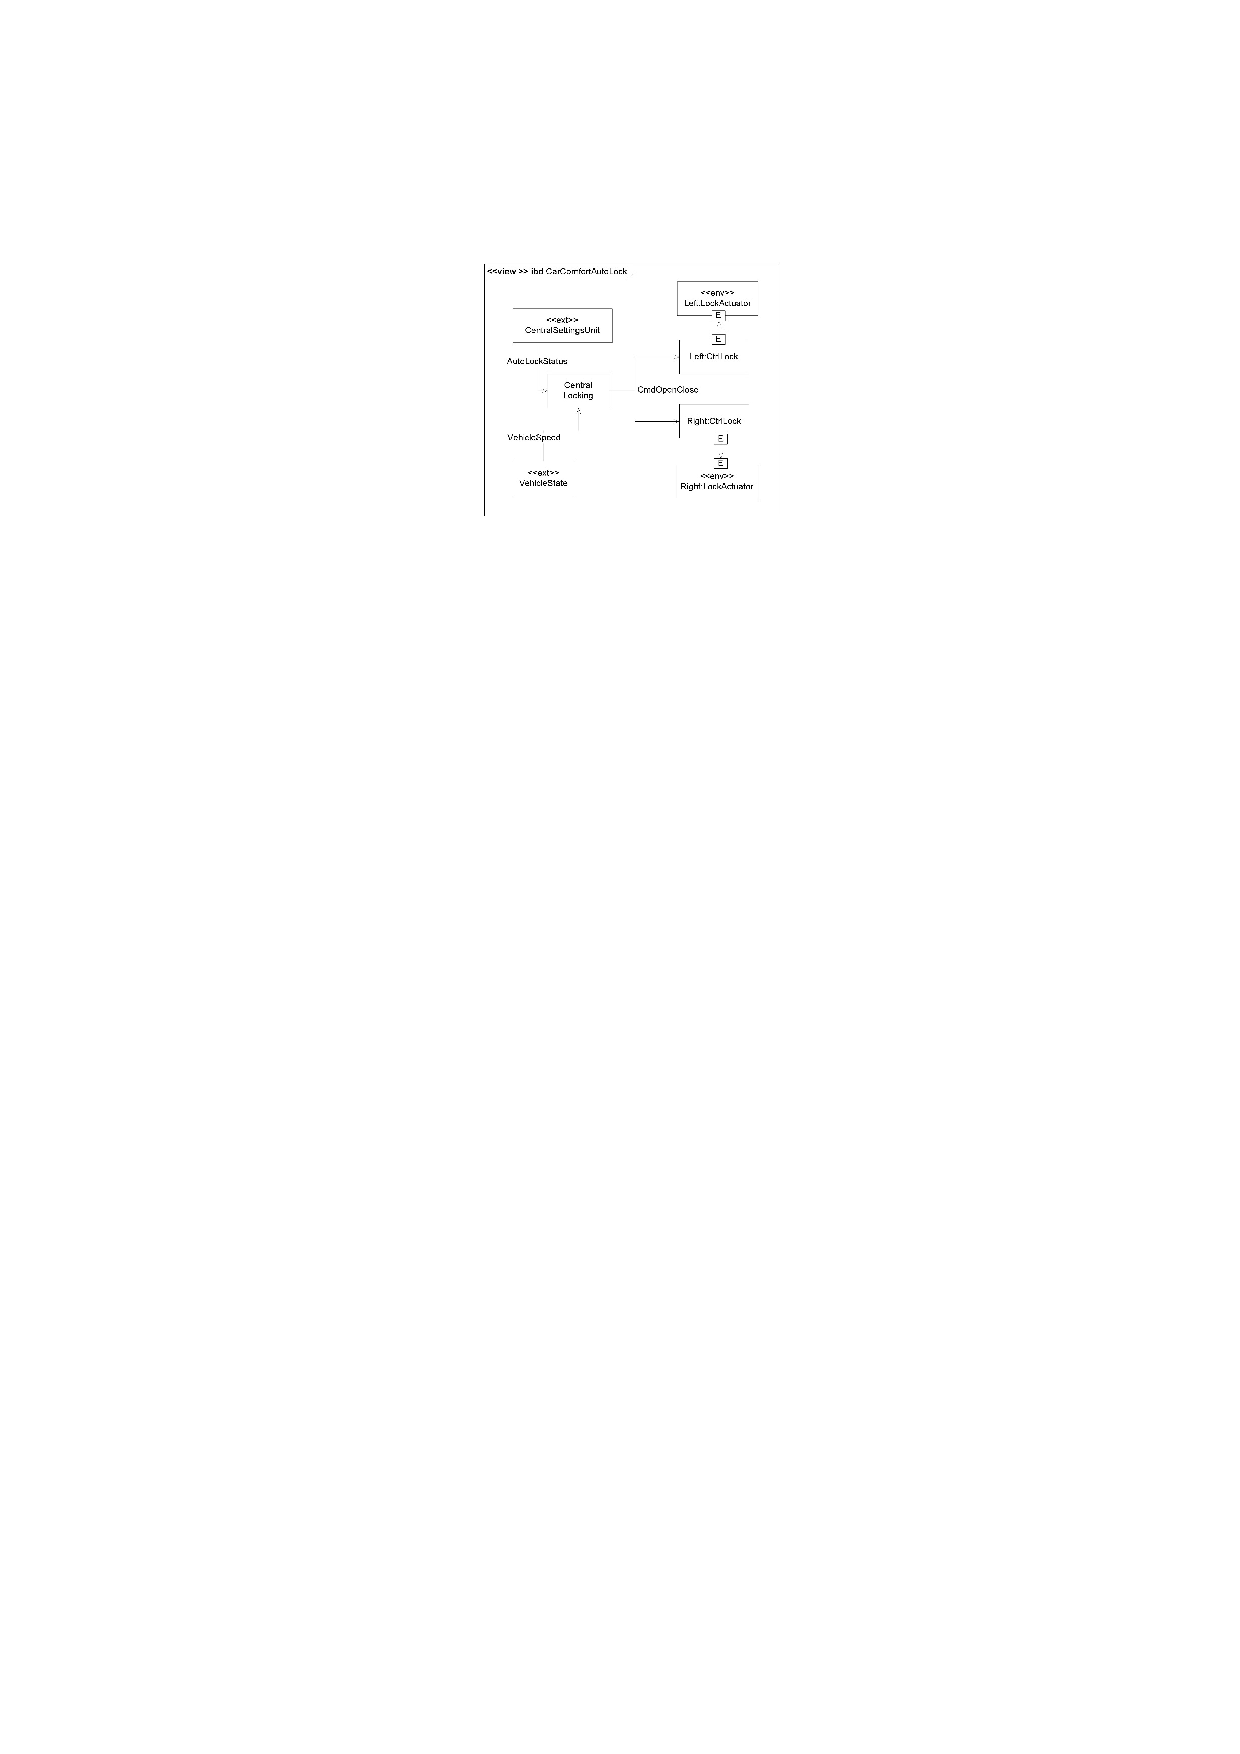
\includegraphics[width=0.35\linewidth]{figure/literatures/gronniger_sysml2.pdf}
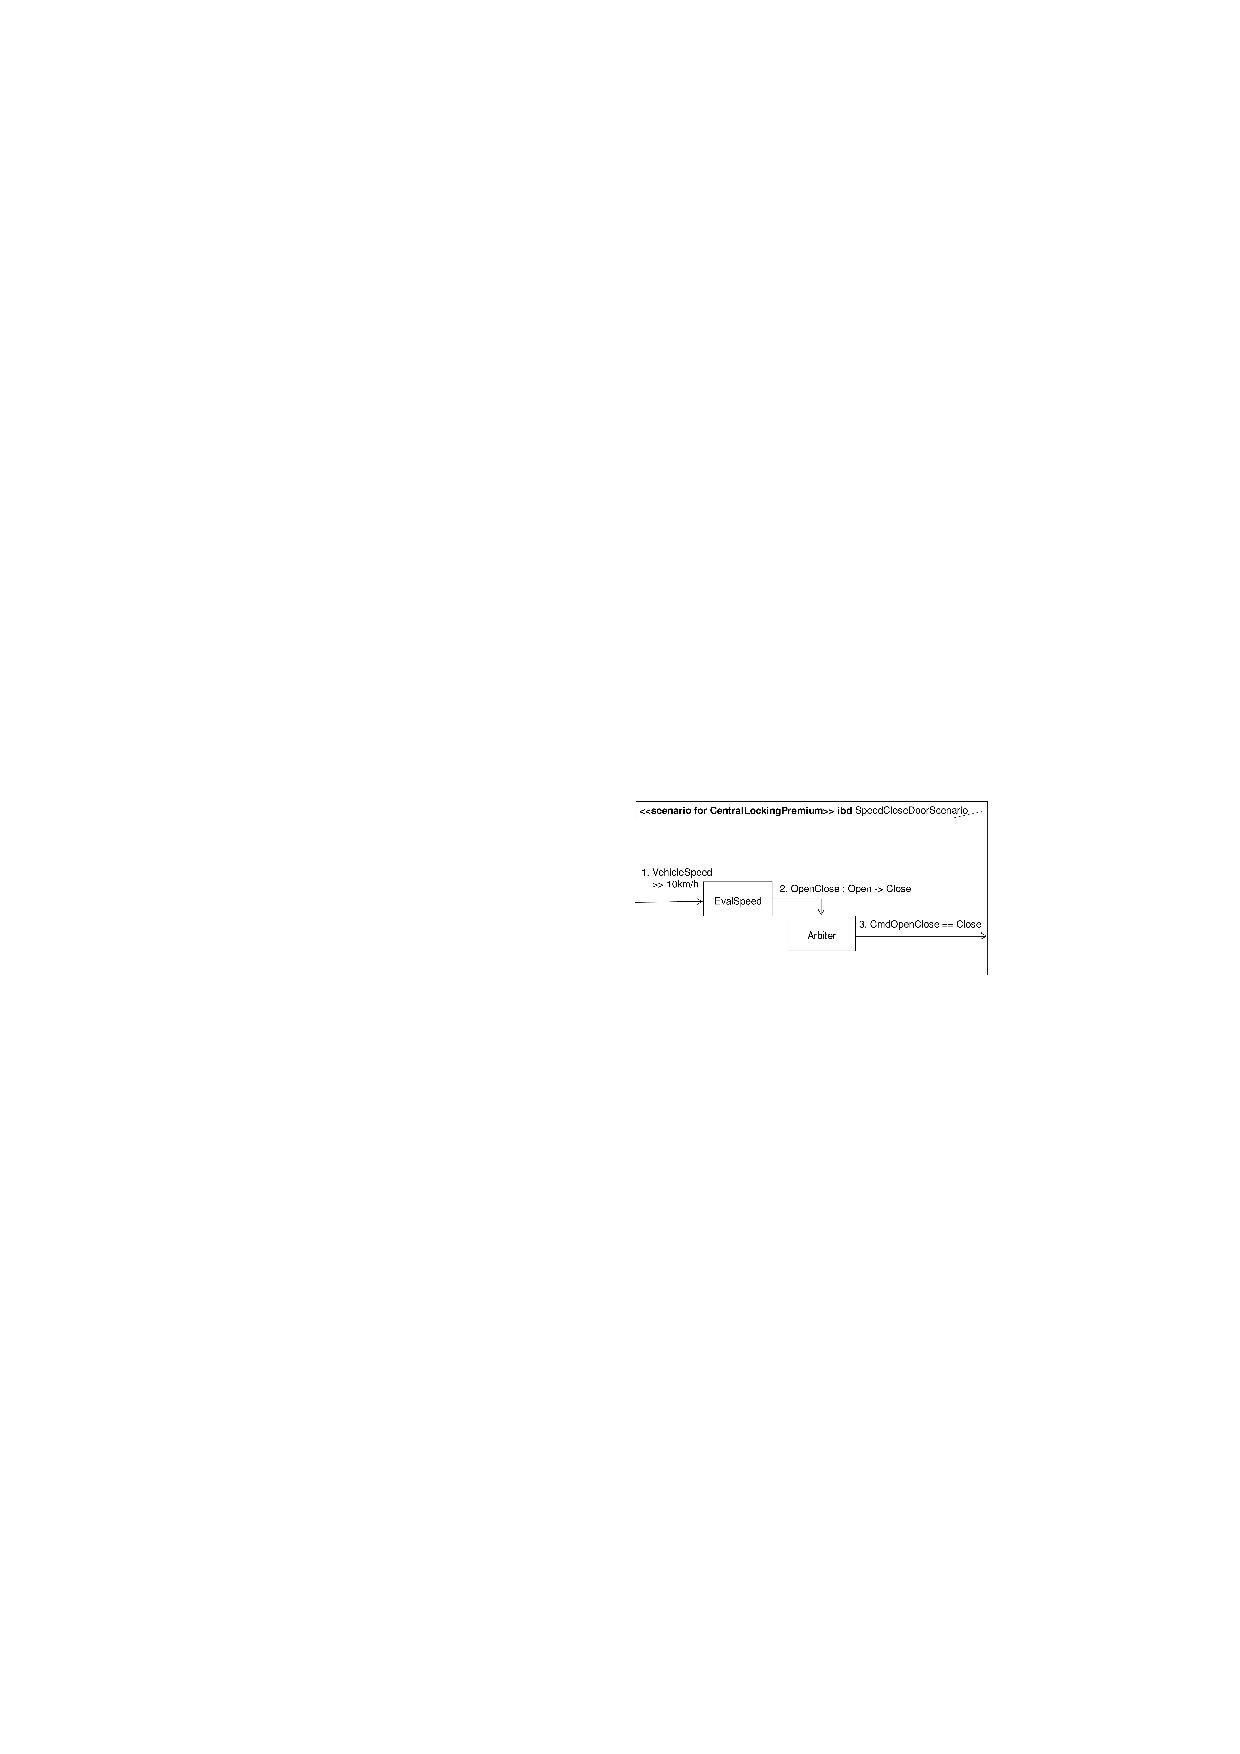
\includegraphics[width=0.5\linewidth]{figure/literatures/gronniger_sysml3.pdf}
\caption{Examples of a functional net \texttt{CarComfort} (top left), a view \texttt{CarComfortAutoLock} (top right), and a scenario \texttt{SpeedClosedDoorScenario} (bottom) \cite{Grönniger}}
\label{fig:gronniger_sysml}
\end{figure}

The authors claim that function nets and views can be used to describe and explain scenarios of use-cases like how an automotive system reacts to external events or failures caused by subsystems (see figure \ref{fig:gronniger_sysml}). However, number of models have to be created as well as references between these models. The authors states in their work that an investigation of existing model management strategies to handle number of models will be performed in the future.\\

Dajsuren \cite{Dajsuren} presents a research which is part of Hybrid innovations of Trucks and it covers the automotive Architecture Description Language (ADL) and quality of automotive software. This research has a role of identifying a proper ways of developing automotive software. \\

The author suggests that automotive software development enables interaction between different engineering fields such as mechanical engineering, electrical engineering and software engineering. ADL can be said to be an effective way to manage such multi-disciplinary engineering information. It has been defined on this paper as ``one of the approach to formalize the representation of the automotive systems and software architecture''. Examples of ADL used in automotive companies are definition of AML for BMW company, EAST-ADL and TADL for Volvo, Fiat, and VW/Carmeq. \\

\begin{figure}[H]
\centering
\captionsetup{justification=centering}
\vspace{0cm}% Adjust vertical spacing here
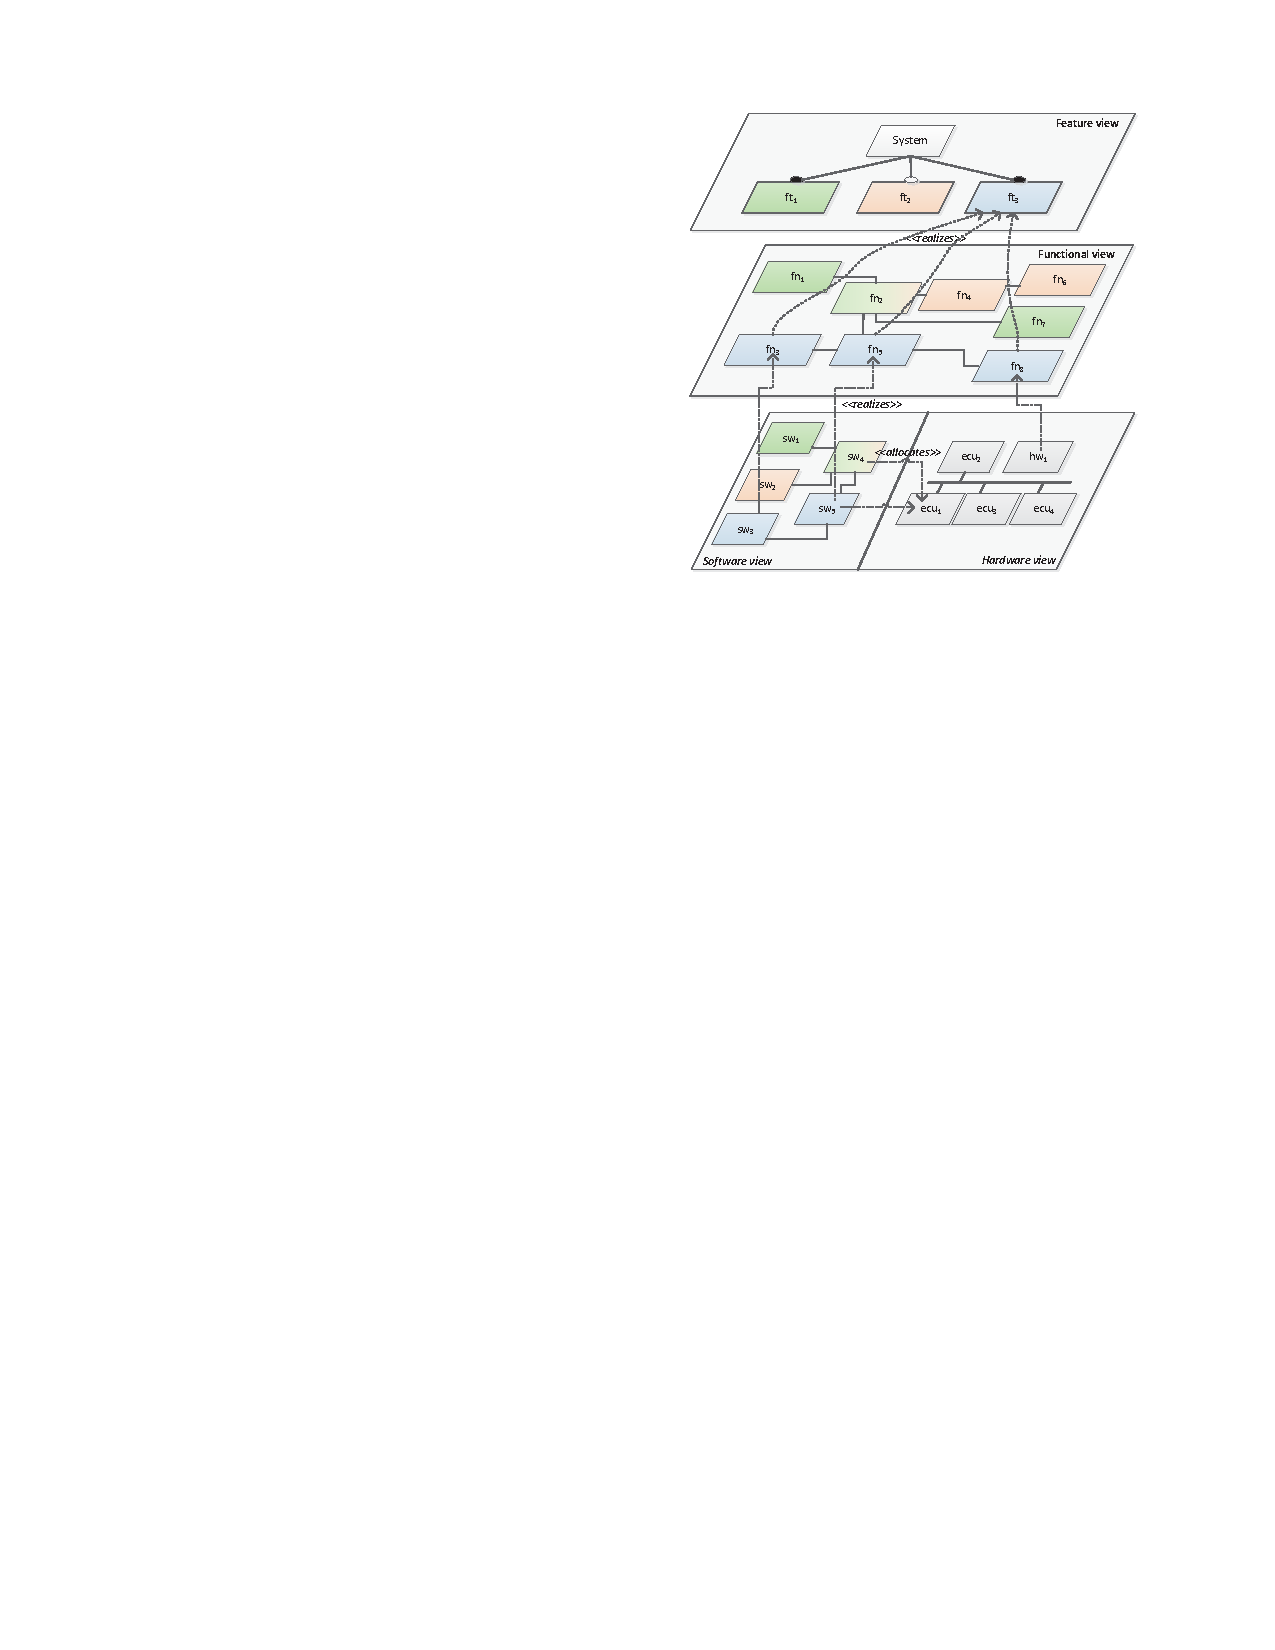
\includegraphics[width=0.5\linewidth]{figure/literatures/dajsuren_adl.pdf}
\caption{Architectural views of an automotive system \cite{Dajsuren}}
\label{fig:dajsuren_adl}
\end{figure}

The different levels of the architecture have been mentioned as well, these include:
\begin{itemize}
    \item \textit{Feature view} that shows number of features in a system.
    \item \textit{Function view} that shows a number of functions or subsystems in a system. A single feature could include one or more function.
    \item \textit{Software view} that shows a detailed architecture. It shows components and blocks which represent the implementation of the functions specified in the function view.
    \item \textit{Hardware view} that contains ECUs, sensors, actuators and Controller Area Network (CAN).
\end{itemize}
\vspace{0.2cm}
The author decided to use and ADL language SysML\footnote{https://sysml.org} in modelling a functional architecture (view) and MATLAB/Simulink has also been mentioned as one of the most popular graphical modelling language and a simulation tool for modelling software architecture (view). \\

The inconsistency of architecture in multiple views has also been explained. This is one of the problem that VCG also experiences which is in between the high- and low-level architectures. In this paper, a consistency rule has been proposed between the different views of the architecture.\\



\section{Low- and high-level electrical architectures at VCG}
To have a better understanding of how low- and high-level electrical architectures have been constructed and used in VCG. The team studied some related works that were conducted in the company.\\

Eliasson et al. \cite{Eliasson_1} find that VCG and Volvo Group Truck Technology (VGTT) have two types of architectures: a high-level architecture and a working architecture (low-level architecture). The high-level architectures produced by high-level architects contain design decision, principles, rules, and pattern that should govern the overall system. The working architecture produced by low-level architects contains logical components which are broken down from the high-level architecture and more details. The study describes that the working architecture is always kept updated by developers as the product evolve, while the high-level architecture is only updated when the project has started. Because of this reason, the inconsistency between the two architecture occurs. It also suggests that having two different groups of architects results to problems. High-level architects have a thought that the low-level architects are very focused on short-term solutions which make them miss an overall picture of the system, while low-level architects see that another group lacks of understanding of current situation and is too focused on solutions that might be good in long run. \\

From another related work, Eliasson et al. \cite{Eliasson_2} also suggest that the presence of the Architecture Technical Debt (ATD) at the design level at VCG plays an important role on the efficiency of communication between components. In this paper, there is a discovery of the ATD items (architectural violations) such as the misplaced LCs and their impacts on the software development process (see figure \ref{fig:eliasson_atd}). The ATD items together with the inputs from the stakeholders at VCG were used to assist in creating a visual tool which provides a better visualization of the ATD items and its interest. With this tool, the visualization is more comprehensive to the stakeholders. 

%FIGURE
\begin{figure}[H]
\centering
\captionsetup{justification=centering}
\vspace{0cm}% Adjust vertical spacing here
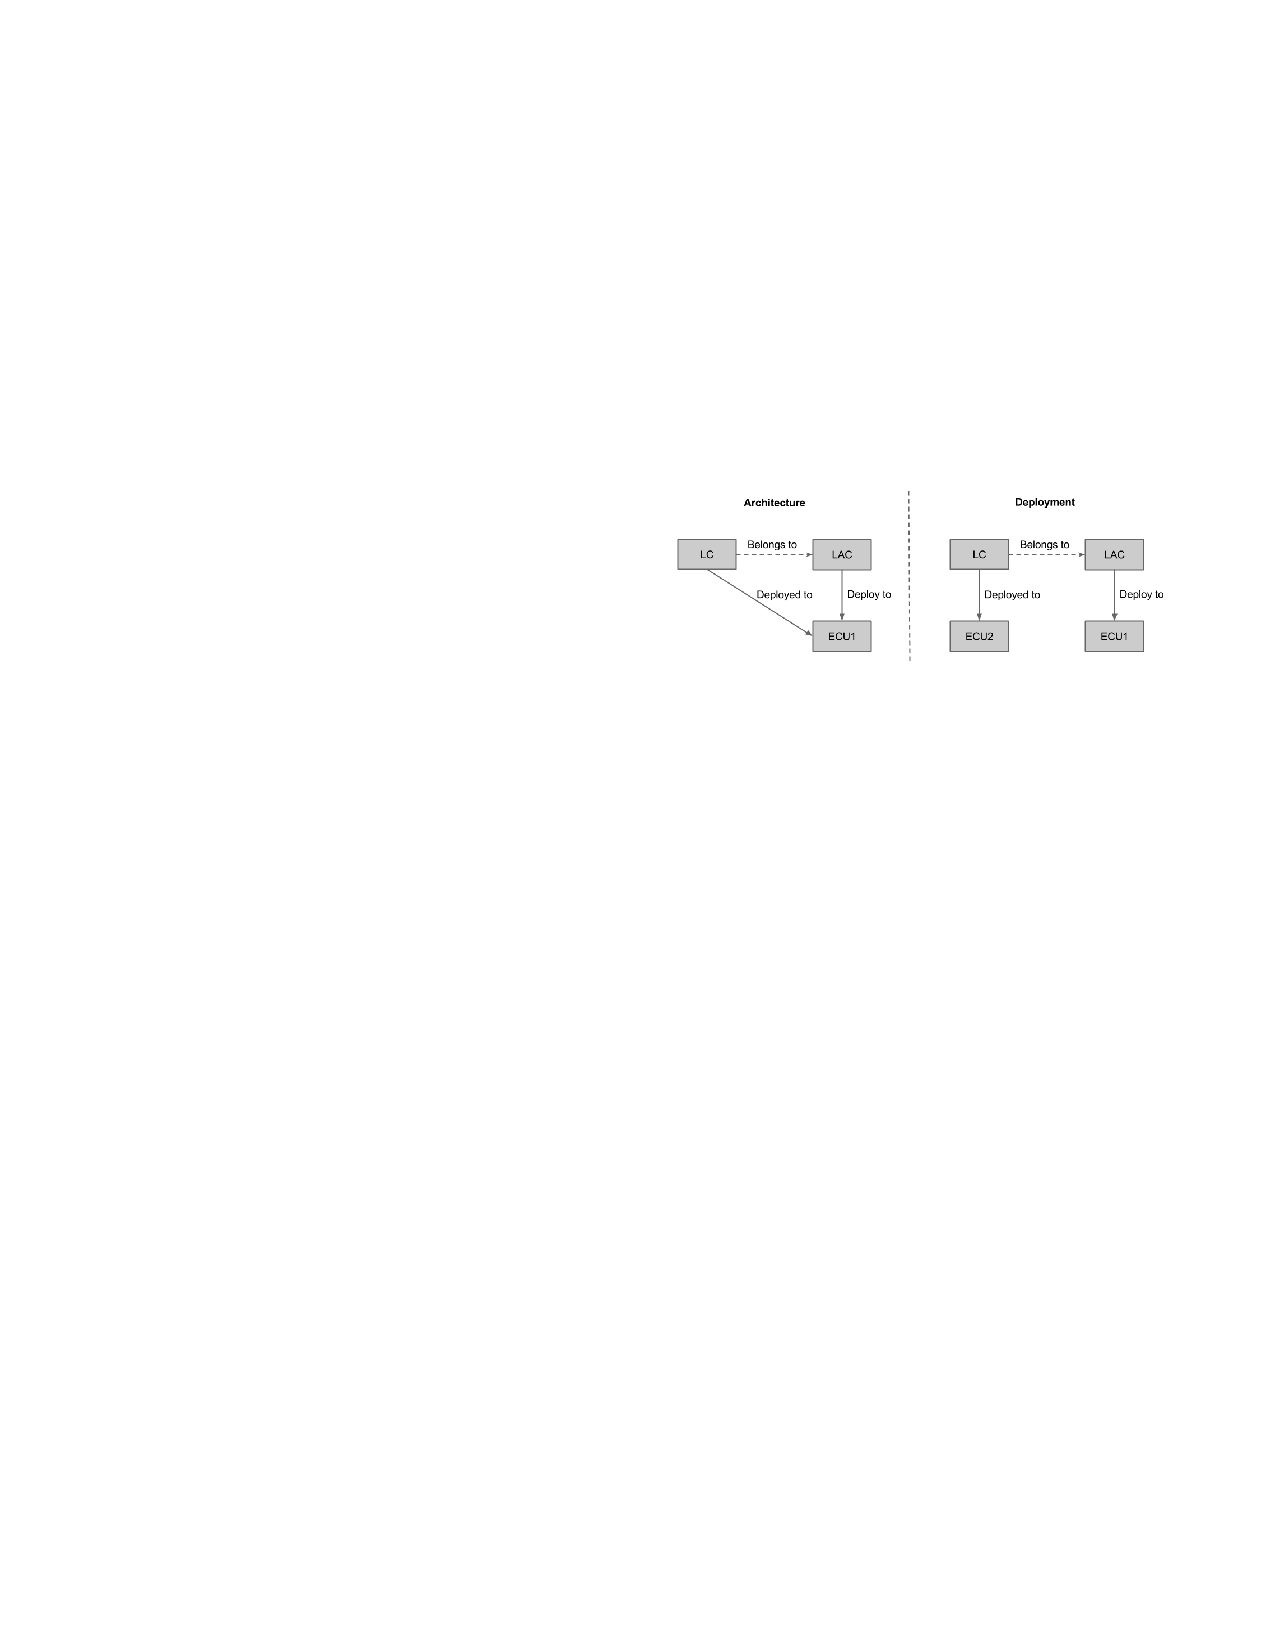
\includegraphics[width=0.7\linewidth]{figure/literatures/eliasson_atd.pdf}
\caption{The difference between architectural design and actual deployment \cite{Eliasson_2}}
\label{fig:eliasson_atd}
\end{figure}


\section{Elektra software and its usage}
At VCG, a custom proprietary tool \textit{Elektra} has been used as a main database storing data related to vehicles such as requirement documents, software components, ECUs, LCs, and LACs. These data are structured similar to directory structure\footnote{The organization of files into hierarchy of folders.} of an operating system, comprising folders and sub-folders. \todo{[to be filled in]}

%FIGURE
\begin{figure}[H]
\centering
\captionsetup{justification=centering}
\vspace{0cm}% Adjust vertical spacing here
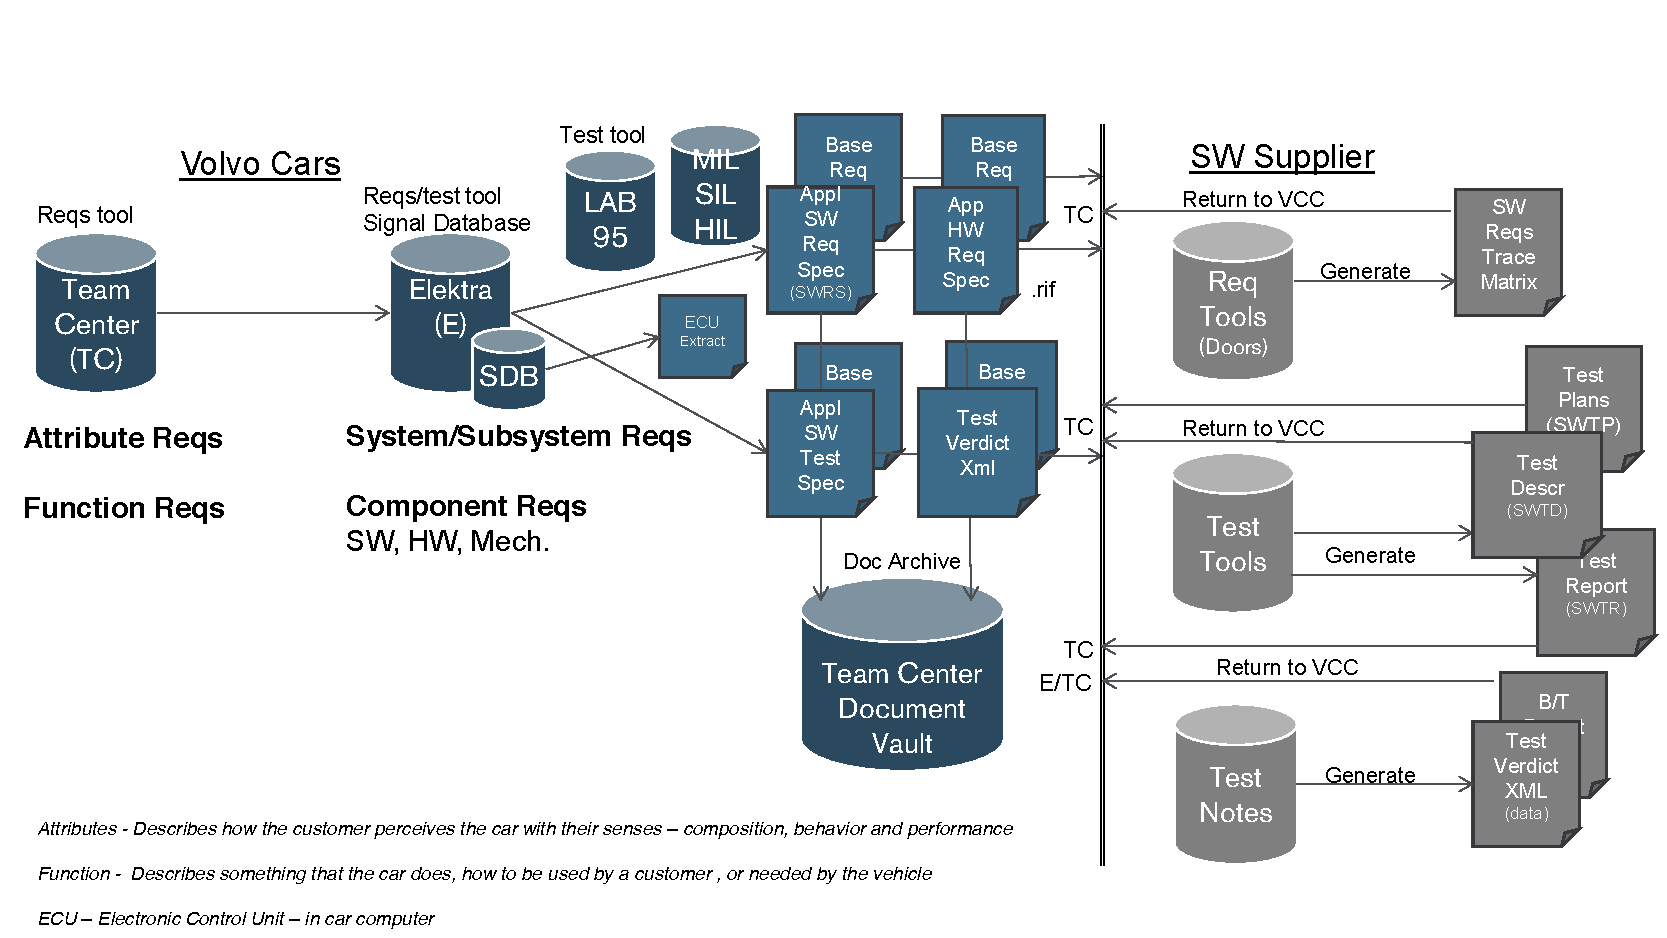
\includegraphics[width=0.95\linewidth]{figure/literatures/niesel_elektra.pdf}
\caption{Diagram showing the tool Elektra acting as a database \cite{Niesel}}
\label{fig:niesel-elektra}
\end{figure}

\section{Data collection method}
One of the key activities of this thesis work is to collect data from stakeholders. the team did some research and found a good method for data collection written by Basili and Weiss \cite{Basili}. The authors developed a goal-oriented data collection method for evaluating software development methodologies. The data that were used in the study were obtained from the changes in 5 software projects developed by different groups with different backgrounds using different development methodologies. They suggest 6 basic steps of data collection as follow:\\[0.1cm]

\begin{step} \label{step:1}
Establishing the goals of the data collection. What are the goals of performing data collection? Why is collecting data needed?
\end{step}

\begin{step} \label{step:2}
Developing a list of questions of interest. What kinds of questions that this study will answer corresponding to the goals in step \ref{step:1}?
\end{step}

\begin{step} \label{step:3}
Establishing data categories. Categories of data must be defined before collecting data.
\end{step}

\begin{step} \label{step:4}
Designing and testing data collection form. A form that is used to collect data must be created before collecting data.
\end{step}

\begin{step} \label{step:5}
Collecting and validating data. Data that are collected must be validated to ensure that they are accurate and complete.
\end{step}

\begin{step} \label{step:6}
Analysing data. Data are analyzed in order to answer the questions in step \ref{step:2}.
\end{step}

Basili and Weiss also suggest that validation of data is a key factor in data gathering. It must be done to ensure ensures correctness, consistency and completeness of data.



\section{Visualization of electrical architectures}
blah blah blah ... \todo{[to be filled in]}